\documentclass[10pt, a4paper]{article}[08.12.2015]
\usepackage[german,ngerman]{babel}
\usepackage[utf8]{inputenc}
\usepackage[T1]{fontenc}
\usepackage{hyperref}
\usepackage[normalem]{ulem}
\usepackage{graphicx}
\usepackage{float}


%\setkomafont{section}{\Large\linespread{1}\sffamily}

\begin{document}
  \title{Ein systematischer Vergleich von Verfahren zur funktionellen und
		taxonomischen Klassifikation von metagenomischen Sequenzfragmenten}
  \author{Marie Sophie Briem, Inga Lemme, Sarah Weber}
  \maketitle
  %\date{\today}
  \thispagestyle{empty}
  \newpage
  \setcounter{page}{2}
  \newpage
  \tableofcontents
  \newpage
  \listoffigures
  \newpage
 % \pagenumbering{arabic}
   \section{Einleitung}
    Der Forschungsbereich der Metagenomik besch\"aftigt sich mit der Klassifizierung und Zuordnung aller genetischen Informationen, die in zuf"allig entnommenen Proben (z.B. marine microbielle Wasser- oder Bodenproben) enthalten sind \cite{handelsman1998}. Aus diesen Proben wird die gesamte enthaltene DNA extrahiert und sequenziert. Anschlie{\ss}end werden die Proteine annotiert um Funktion und Taxonomie der enthaltenden Spezies zu ermitteln (Abb.1).
    Basierend auf neuen und schnellen Sequenzierverfahren wie Illumina, fallen aus der Metagenomik gro{\ss}e Datenmengen an, die taxonomisch und funktionell klassifiziert werden m\"ussen. Eine vielversprechende Alternative zu dem Alignierprogramm BlastX, welches mithilfe von Sequenzvergleichen eine solche Klassifizierung durchf\"uhrt, scheinen Diamond \cite{buchfink2014} und Lambda \cite{hauswedell2014} zu sein, die eine Laufzeitersparnis mit Hilfe von double indexing erwirken sollen. 
    \newline
    \begin{figure}[h]
\centering
      \noindent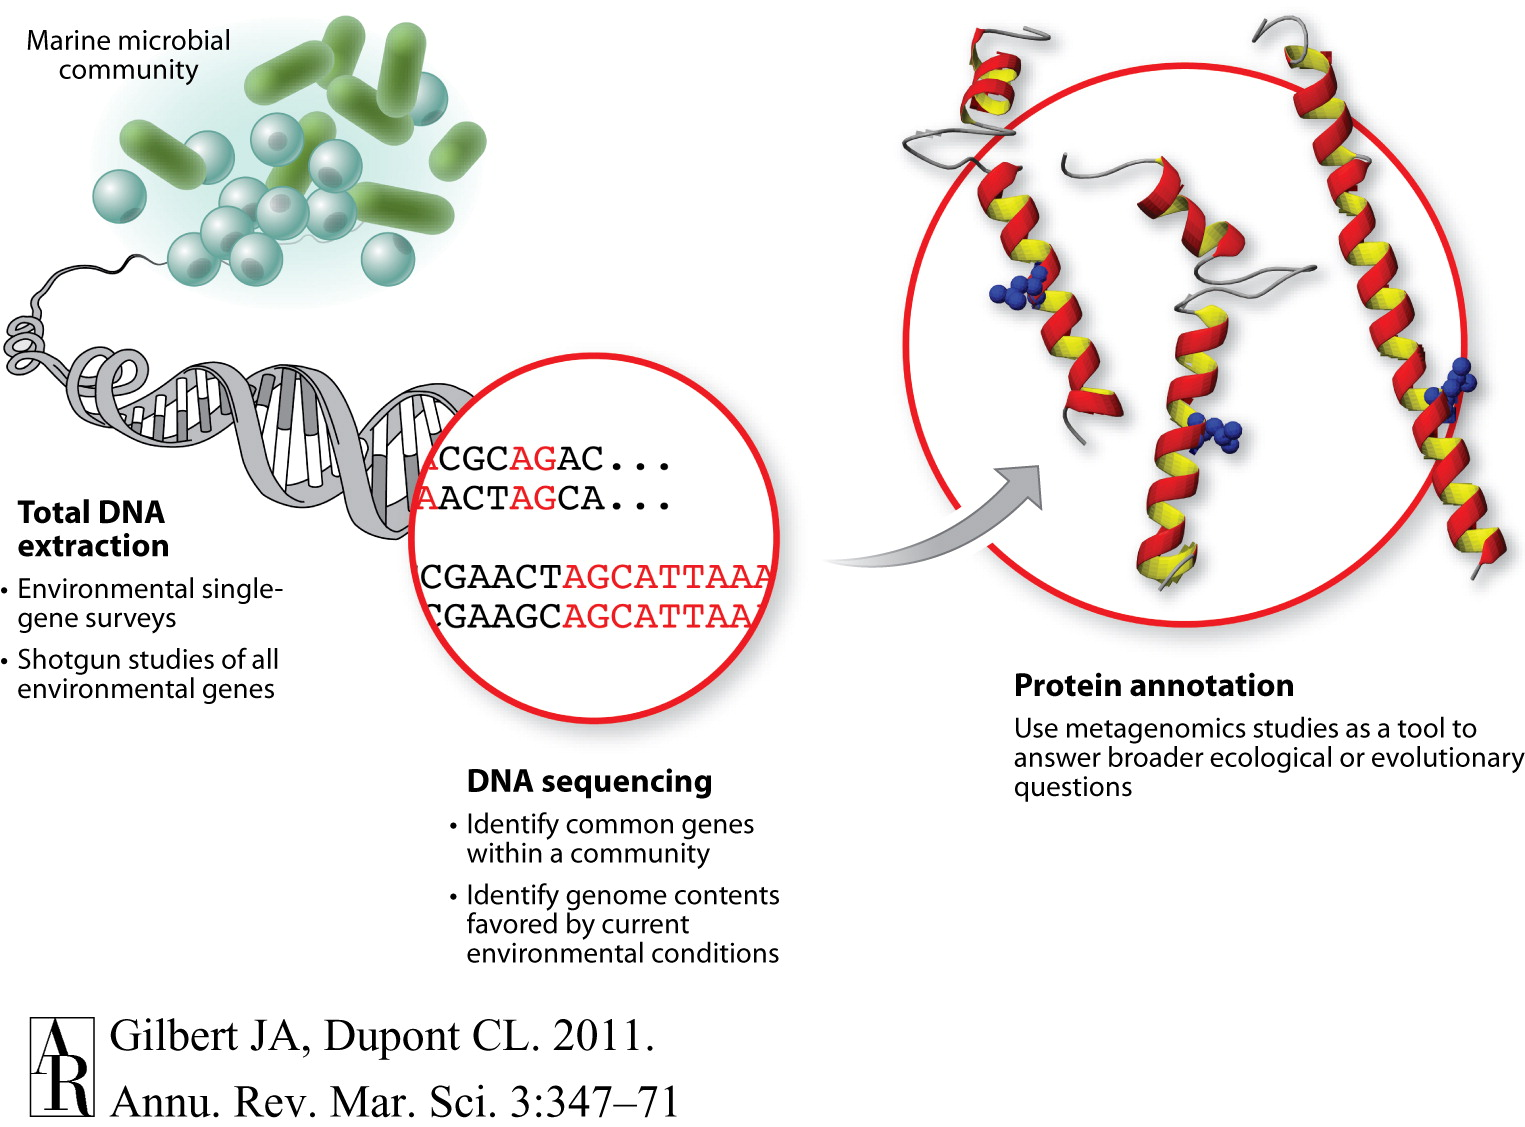
\includegraphics[width=\linewidth,height=15cm,
      keepaspectratio]{Abbildungen/metagenome-steps.jpg}
      \caption{Metagenomik in Schritten}
\end{figure}
\newline    
    
    \subsection{\textrm{Diamond}}    
    Das open source verf\"ugbare Alignierprogramm Diamond \cite{buchfink2014} basiert auf einem Seed- und Extent Algorithmus. Im Seedingschritt werden so gennante Spaced Seeds gesucht, die als Treffer in Anfrage- und Datenbanksequenz gefunden werden sollen (Abb. 2). Das Seeding findet anschlie{\ss}end mit Double Indexing statt. Beim Double Indexing werden sowohl Anfrage- als auch Referenzdatenbanksequenz geindext, was eine geringere Laufzeit durch schnelleres durchsuchen der Datenstrukturen mit sich bringt. Die Indizierung findet bei Diamond $"$on the fly$"$, das hei{\ss}t w\"ahrend des Programmdurchlaufs, statt. Die Treffer, die mit Hilfe der Spaced Seeds gefunden wurden, speichert Diamond in lexikographisch sortierten Listen.
\begin{figure}[h]
\centering
      \noindent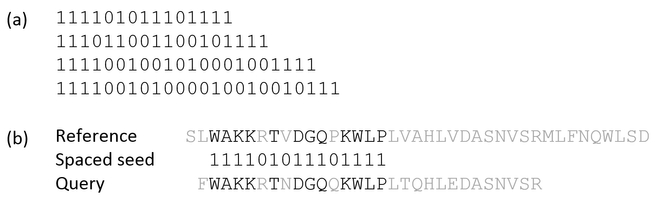
\includegraphics[width=\linewidth,height=15cm,
      keepaspectratio]{Abbildungen/diamond_spacedSeeds.jpg}
      \caption{Spaced Seeds}
\end{figure}
\newline
    Um eine Erweiterung im Extendschritt durchzuf\"uhren, \"uberpr\"uft das Programm, ob der Seed-Treffer gr\"o{\ss}er-gleich 10 Aminos\"auren lang ist. Der Seed wird schlie{\ss}lich mit dem Smith-Waterman Algorithmus erweitert.
\newline
    
    \subsection{\textrm{Lambda}}
    Auch Lambda \cite{hauswedell2014} basiert wie Diamond auf dem Seed- und Extend Algorithmus mit Double Indexing. Im Gegensatz zu Lambda muss die Refernzdatenbank vorgeindext werden und findet nicht w\"ahrend des Programmdurchlaufs statt. Als Datenstrukturen stehen f\"ur die Referenzdatenbank ein Suffixarray und f\"ur die Anfragesequenz ein Radixtree zur Verf\"ugung. Die Speicherung in einem Radixtree erm\"oglicht eine Paralellisierung verschiedener Seeds, was eine zus\"atzliche Zeitersparnis bedeutet. 
    Die Erweiterung erflolgt mit Hilfe des X-drop Algorithmus. 
    \subsection{Ziele}
    
    Das Projekt hat folgende Ziele:
    
    \begin{itemize}
    
      \item Bestimmung und Vergleich der Sensivit"at (Anzahl an korrekt Bestimmten / Anzahl an Sequenzen im Datenset) und Pr\"azision (Anzahl an korrekt Bestimmten / Anzahl an Zugewiesenen) der Programme \textrm{Diamond} 				und \textrm{Lambda}.
      
      \item Bestimmung und Vergleich der ben"otigten Zeit der Programme
      		\textrm{Diamond} und \textrm{Lambda}.

      
    
    \end{itemize}


    \newpage
  \section{Material und Methoden}
    
    \subsection{Material} 
    
      Das durchgef"uhrte Projekt orientiert sich an der Forschungsarbeit von
      Bazinet und Cummings \cite{bazinet2012}. Im 
      Folgenden bezieht sich der Ausdruck "Vorlagepaper"\ auf die Arbeit von
      Bazinet und Cumming. Die Datensets und Datenbanken wurden anhand des 			  Vorlagepapers ausgew"ahlt.
      
      \subsubsection{Datensets}
        Die Experimente wurden mit folgenden Datensets durchgef"uhrt:
        
        \begin{enumerate}
        
          \item \textit{FACS 269bp} $-$ Datenset, original von Strannenheim 			  \textit{et al.} \cite{stranneheim2010}, bestehend aus
          \textbf{27.049 simulierten 454 
          Reads} mit einer durschnittlichen L"ange von \textbf{269 bp}. Die
          im Vorlagepaper angegebene Referenz war nicht mehr aktuell und
          konnte nicht gefunden werden. Das
          Datenset wurde direkt von Herrn Bazinet bereit gestellt. Das 					  bereitgestellte Datenset beinhaltet 72.951 Reads der Spezies 					  \textit{Homo sapiens}. Diese Reads wurden entfernt, so dass das 				  genutzte Datenset 27.049 Reads enth\"alt. Das Datenset setzt sich aus 		  19 bakteriellen und drei viralen Genomen zusammen 							  \cite{bazinet2012}.  
           
          \item \textit{CARMA 265bp} $-$ Datenset bestehend aus
          \textbf{25.000 simulierten 454 Reads} mit einer durschnittlichen 				  L"ange von \textbf{265 bp}, original genutzt von Gerlach und Stoye
          \cite{GerlachStoye2011}.
          Das Datenset
          wurde von der WebCARMA Homepage unter dem Link
          \url{http://wwww.cebitec.uni-bielefeld.de/webcarma.cebitec.uni-
          bielefeld.de/download/simulated_metagenome_454_265bp.fna}\newline
          heruntergeladen. Zusammengesetzt ist das Datenset aus 25 bakteriellen
          Genomen, die sich wie folgt in die einzelnen bakteriellen Phyla 				  verteilen: 73,0\% Proteobacteria; 12,9\% Firmicutes; 7,8\% 					  Cyanobacteria; 5,2\% Actinobacteria; 1,0\% Clamydiae 							  \cite{bazinet2012}.
          
          \item \textit{Metaphyler 300bp} $-$ Datenset bestehend aus 
          \textbf{73.086 simulierten
          Reads} von 31 phylogenetischen Markern bakterieller Genome mit 			  	  einer durschnittlichen L"ange von \textbf{300 bp}. Urspr\"unglich 			  genutzt von Liu \textit{et al.} \cite{Liu2010}. Das
          Datenset konnte anhand der im Vorlagepaper angegebenen Referenz nicht 
          korrekt ermittelt werden. Die Rechercheergebnisse
          ergaben ein Datenset bestehend aus 40.039 Reads mit einer 
          durchschnittlichen L"ange von 645 bp. Das korrekte
          Datenset wurde direkt von Herrn Bazinet bereit gestellt. 
          Die Verteilung in die bakteriellen Phyla setzt sich folgenderma"sen 			  zusammen: 47.0\% Proteobacteria; 21.9\% Firmicutes; 9.7\% 					  Actinobacteria; 4.8\% Bacteroidetes; 3.9\% Cyanobacteria; 2.2\% 				  Tenericutes; 1.9\% Spirochaetes; 1.3\% Chlamydiae; 0.9\% 						  Thermotogae; 0.9\% Chlorobi \cite{bazinet2012}. 
          
          \item \textit{PhymmBL 243bp} $-$ Datenset bestehend aus 
          \textbf{80.215 RefSeq
          Reads} mit einer durschnittlichen L"ange von
          \textbf{243 bp}. Das Datenset, original genutzt von Brady und 
          Salzberg \cite{bradysalzberg2009},  
          konnte anhand der im Vorlagepaper angegebenen Referenz nicht 
          korrekt ermittelt werden. Die Rechercheergebnisse
          ergaben ein Datenset bestehend aus 73.252 Reads mit einer 
          durchschnittlichen L"ange von 204 bp. Das korrekte
          Datenset wurde direkt von Herrn
          Bazinet bereit gestellt.  
          
          \item \textit{PhyloPythia 969bp} $-$ simMC Datenset bestehend aus
          \textbf{114.457 Reads} mit einer durschnittlichen L"ange von
          \textbf{969 bp}, original von Patil \textit{et al.} \cite{patil2011}. 		  Das im Vorlagepaper verwendete Datenset 
          "PhyloPythia"\ bestehend aus 124.941 Reads mit einer 
          durchschnittlichen L"ange von 961 bp konnte
          auch mit Hilfe von Herrn Bazinet nicht ermittelt werden.
          Das Datenset wurde von der JGI Homepage unter dem Link
          \url{http://fames.jgi-psf.org/Retrieve_data.html} heruntergeladen.  
          
          \item \textit{RAIphy 233bp} $-$ Datenset bestehend aus
          \textbf{477.000 RefSeq Reads} mit einer durschnittlichen L"ange von
          \textbf{233 bp}, original von Nalbantoglu \textit{et al.} 					  \cite{nalbantoglu2011}. Das im Vorlagepaper verwendete Datenset 
          "RAIphy"\ bestehend aus 477.000 Reads mit einer 
          durchschnittlichen L"ange von 238 bp konnte
          mit der angegebenen Referenz nicht ermittelt werden.
          Das im Projekt verwendete Datenset wurde von Herrn Bazinet zur
          Verf"ugung gestellt.
          
        \end{enumerate}
        
      \subsubsection{Datenbank}
      F\"ur die Suche wurde die Datenbank UniProtKB/Swiss-Prot von UniProt 			  verwendet \cite{bairoch2004}.
      Diese wurde unter dem Link \url{http://www.uniprot.org/downloads}
      heruntergeladen.
      Die Datenbank besteht aus 549.646 Sequenzen mit einer durchschnittlichen 
      L\"ange von 356.56bp.
      \subsubsection{Programme}
        Im Projekt wurden folgende Programme verwendet:
        
        \begin{enumerate}
          
          \item \textbf{Lambda} $-$ Das Programm Lambda (Version 0.9.2) wurde 			  von der GitHub Seite mit dem Link 											  \url{https://github.com/seqan/lambda.git} heruntergeladen 					  \cite{hauswedell2014}. Dabei wurde wie folgt vorgegangen:
          \begin{itemize}
            \item[\$] git clone \url{https://github.com/seqan/lambda.git}
            \item[\$] cd lambda
            \item[\$] mkdir build
            \item[\$] cmake 																    -DCMAKE\_C\_COMPILER=/usr/local/zbhtools/gcc/gcc-5.1.0/bin/gcc 
            -DCMAKE\_CXX\_COMPILER=/usr/local/zbhtools/gcc/gcc-5.1.0/bin/g++ 
            -DCMAKE\_INSTALL\_PREFIX=\$/work/gi/software 
            \item[\$] make -j2													   
          \end{itemize}
          Um das Programm Lambda ausf\"uhren zu k\"onnen musste die 					  UniProtKB/Swiss-Prot Datenbank zun\"achst indiziert werden. Dazu 				  wurde das Programm "lambda\_indexer"\ verwendet, welches in dem oben 			  genannten Packet enthalten ist. Folgender Aufruf wurde verwendet:
          \begin{itemize}
            \item[\$] lambda\_indexer -d uniprot\_sprot.fasta
          \end{itemize}
          Die jeweiligen Datensets (s.o.) wurden gegen die indizierte Datenbank 
          mit dem Befehl
          \begin{itemize}
            \item[\$] lambda -q QUERY.fasta -d DATABASE.fasta [-o output.m8]
          \end{itemize}
          aligniert.
          
          
          \item \textbf{Diamond} $-$ Das Programm Diamond (Version 0.7.9) wurde 
          von der GitHub Seite mit dem Link
          \url{https://github.com/bbuchfink/diamond.git} heruntergeladen
          \cite{buchfink2014}. Es wurde folgenderma\ss{en} verfahren:
          \begin{itemize}
            \item[\$] git clone \url{https://github.com/bbuchfink/diamond.git}
            \item[\$] cd diamond
            \item[\$] mkdir build
            \item[\$] cmake 																-DCMAKE\_INSTALL\_PREFIX=\$/work/gi/software/diamond
            \item[\$] make install
		  \end{itemize}
		  Mit dem Aufruf
		  \begin{itemize}
		    \item[\$] diamond makedb --in uniprot\_sprot.fasta -d 							diamonduniprot\_sprot.fasta.dmnd
		  \end{itemize}
		  wurde die bin\"are Diamond-Datenbank aus der UniProtKB/Swiss-Prot 			  erstellt.\newline
		  Die jeweiligen Datensets (s.o.) wurden gegen die zuvor erstellte 				  Diamond-Datenbank mit dem Befehl
		  \begin{itemize}
		    \item[\$] diamond blastx -d DIAMOND\_DATABASE.dmnd -q QUERY.fasta 				-a OUTPUT -t <temporary directory> 
		  \end{itemize}
		  aligniert.		             
          
          \item \textbf{Megan} $-$
          
        \end{enumerate}
    \subsection{Methoden}
    
  
    \newpage
  \section{Ergebnisse}
  Die Abbildungen 3 - 8 zeigen die Distanzverteilungen der Reads, welche mithilfe des newick-parser ermittelt wurden. Um einen direkten Vergleich von Diamond und Lambda vornehmen zu k\"onnen, wurden pro Datensatz die Verteilungen beider Programme aufgef\"uhrt. Die Datensa\"atze Carma (Abb. 3), Facs (Abb. 4) und PhyloPythia (Abb. 5) zeigen die gemeinsame Tendenz, dass Diamond viele Reads bei kleinen Distanzen aufweist. Die Ausgaben von Lambda zeigen oftmals erst bei einer Distanzgr\"o{\ss}e von > 4 bemerkenswerte Readanzahlen.
  
    \begin{figure}[H]
      \centering
      \noindent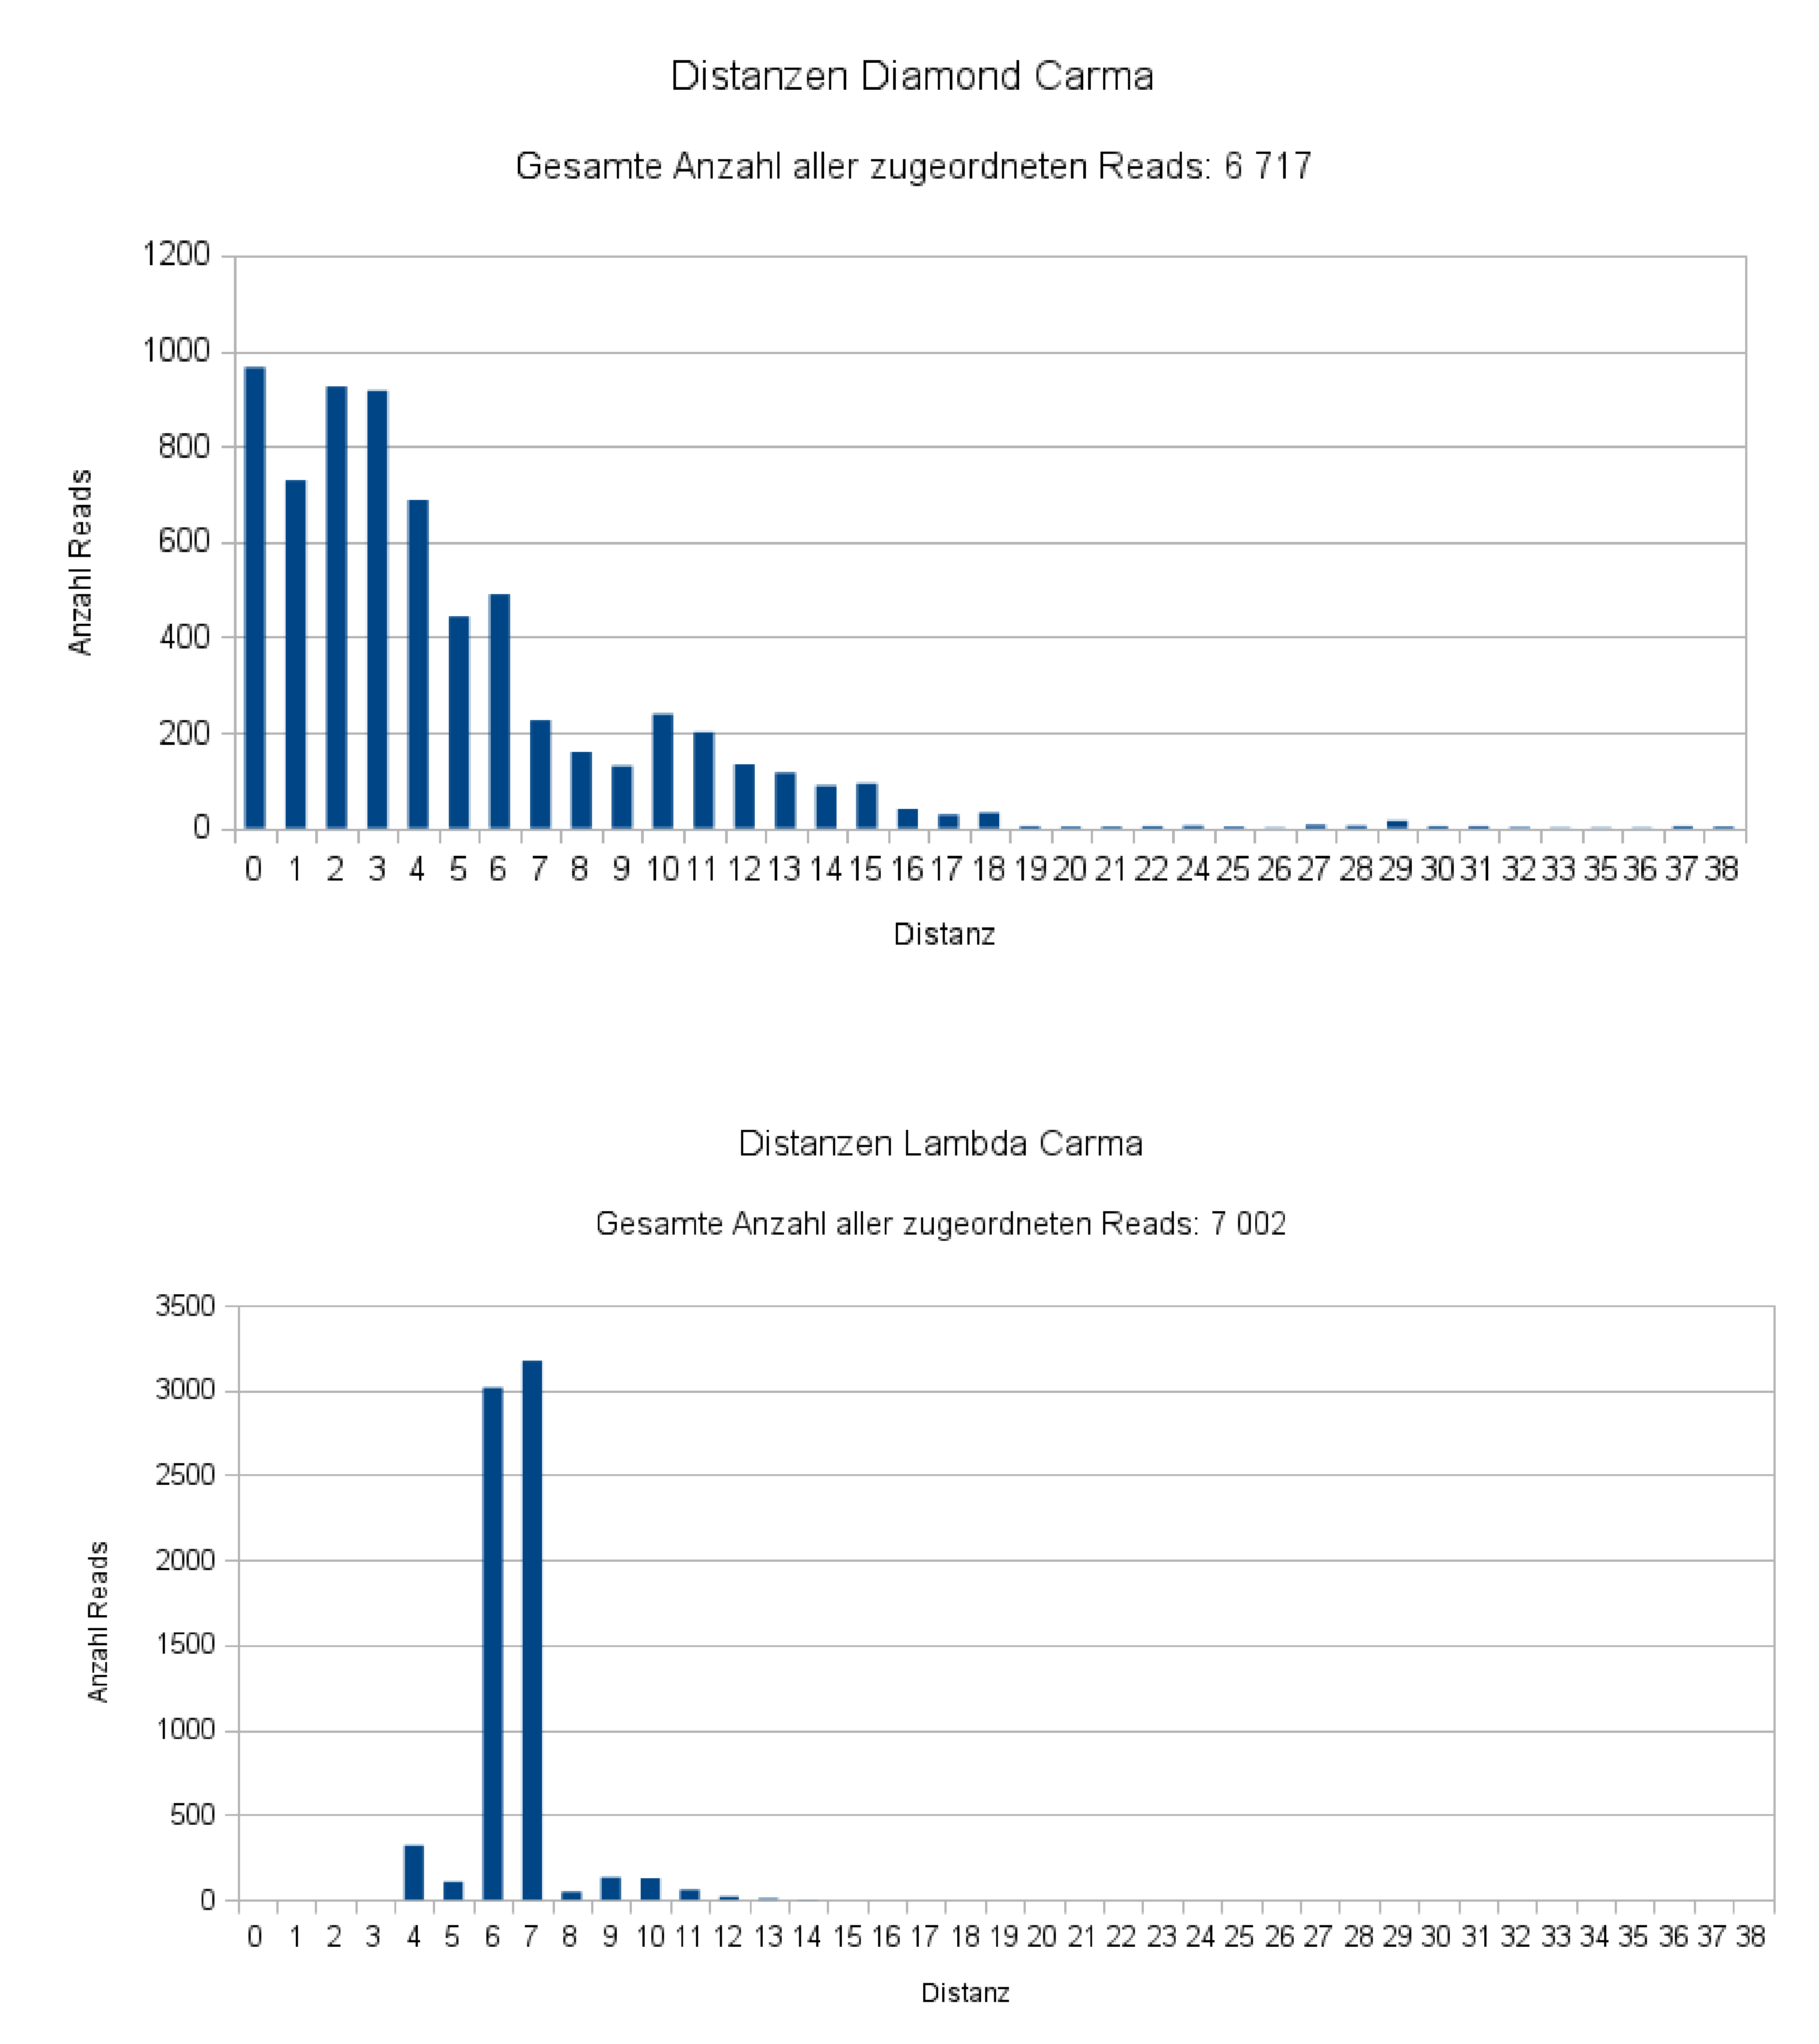
\includegraphics[width=\linewidth,height=15cm,
      keepaspectratio]{Abbildungen/Carma_Distanzen_both.png}
      \caption{Verteilung der Distanzen: Carma Datensatz}
      \centering     
    \end{figure}

    \begin{figure}[H]
      \centering
      \noindent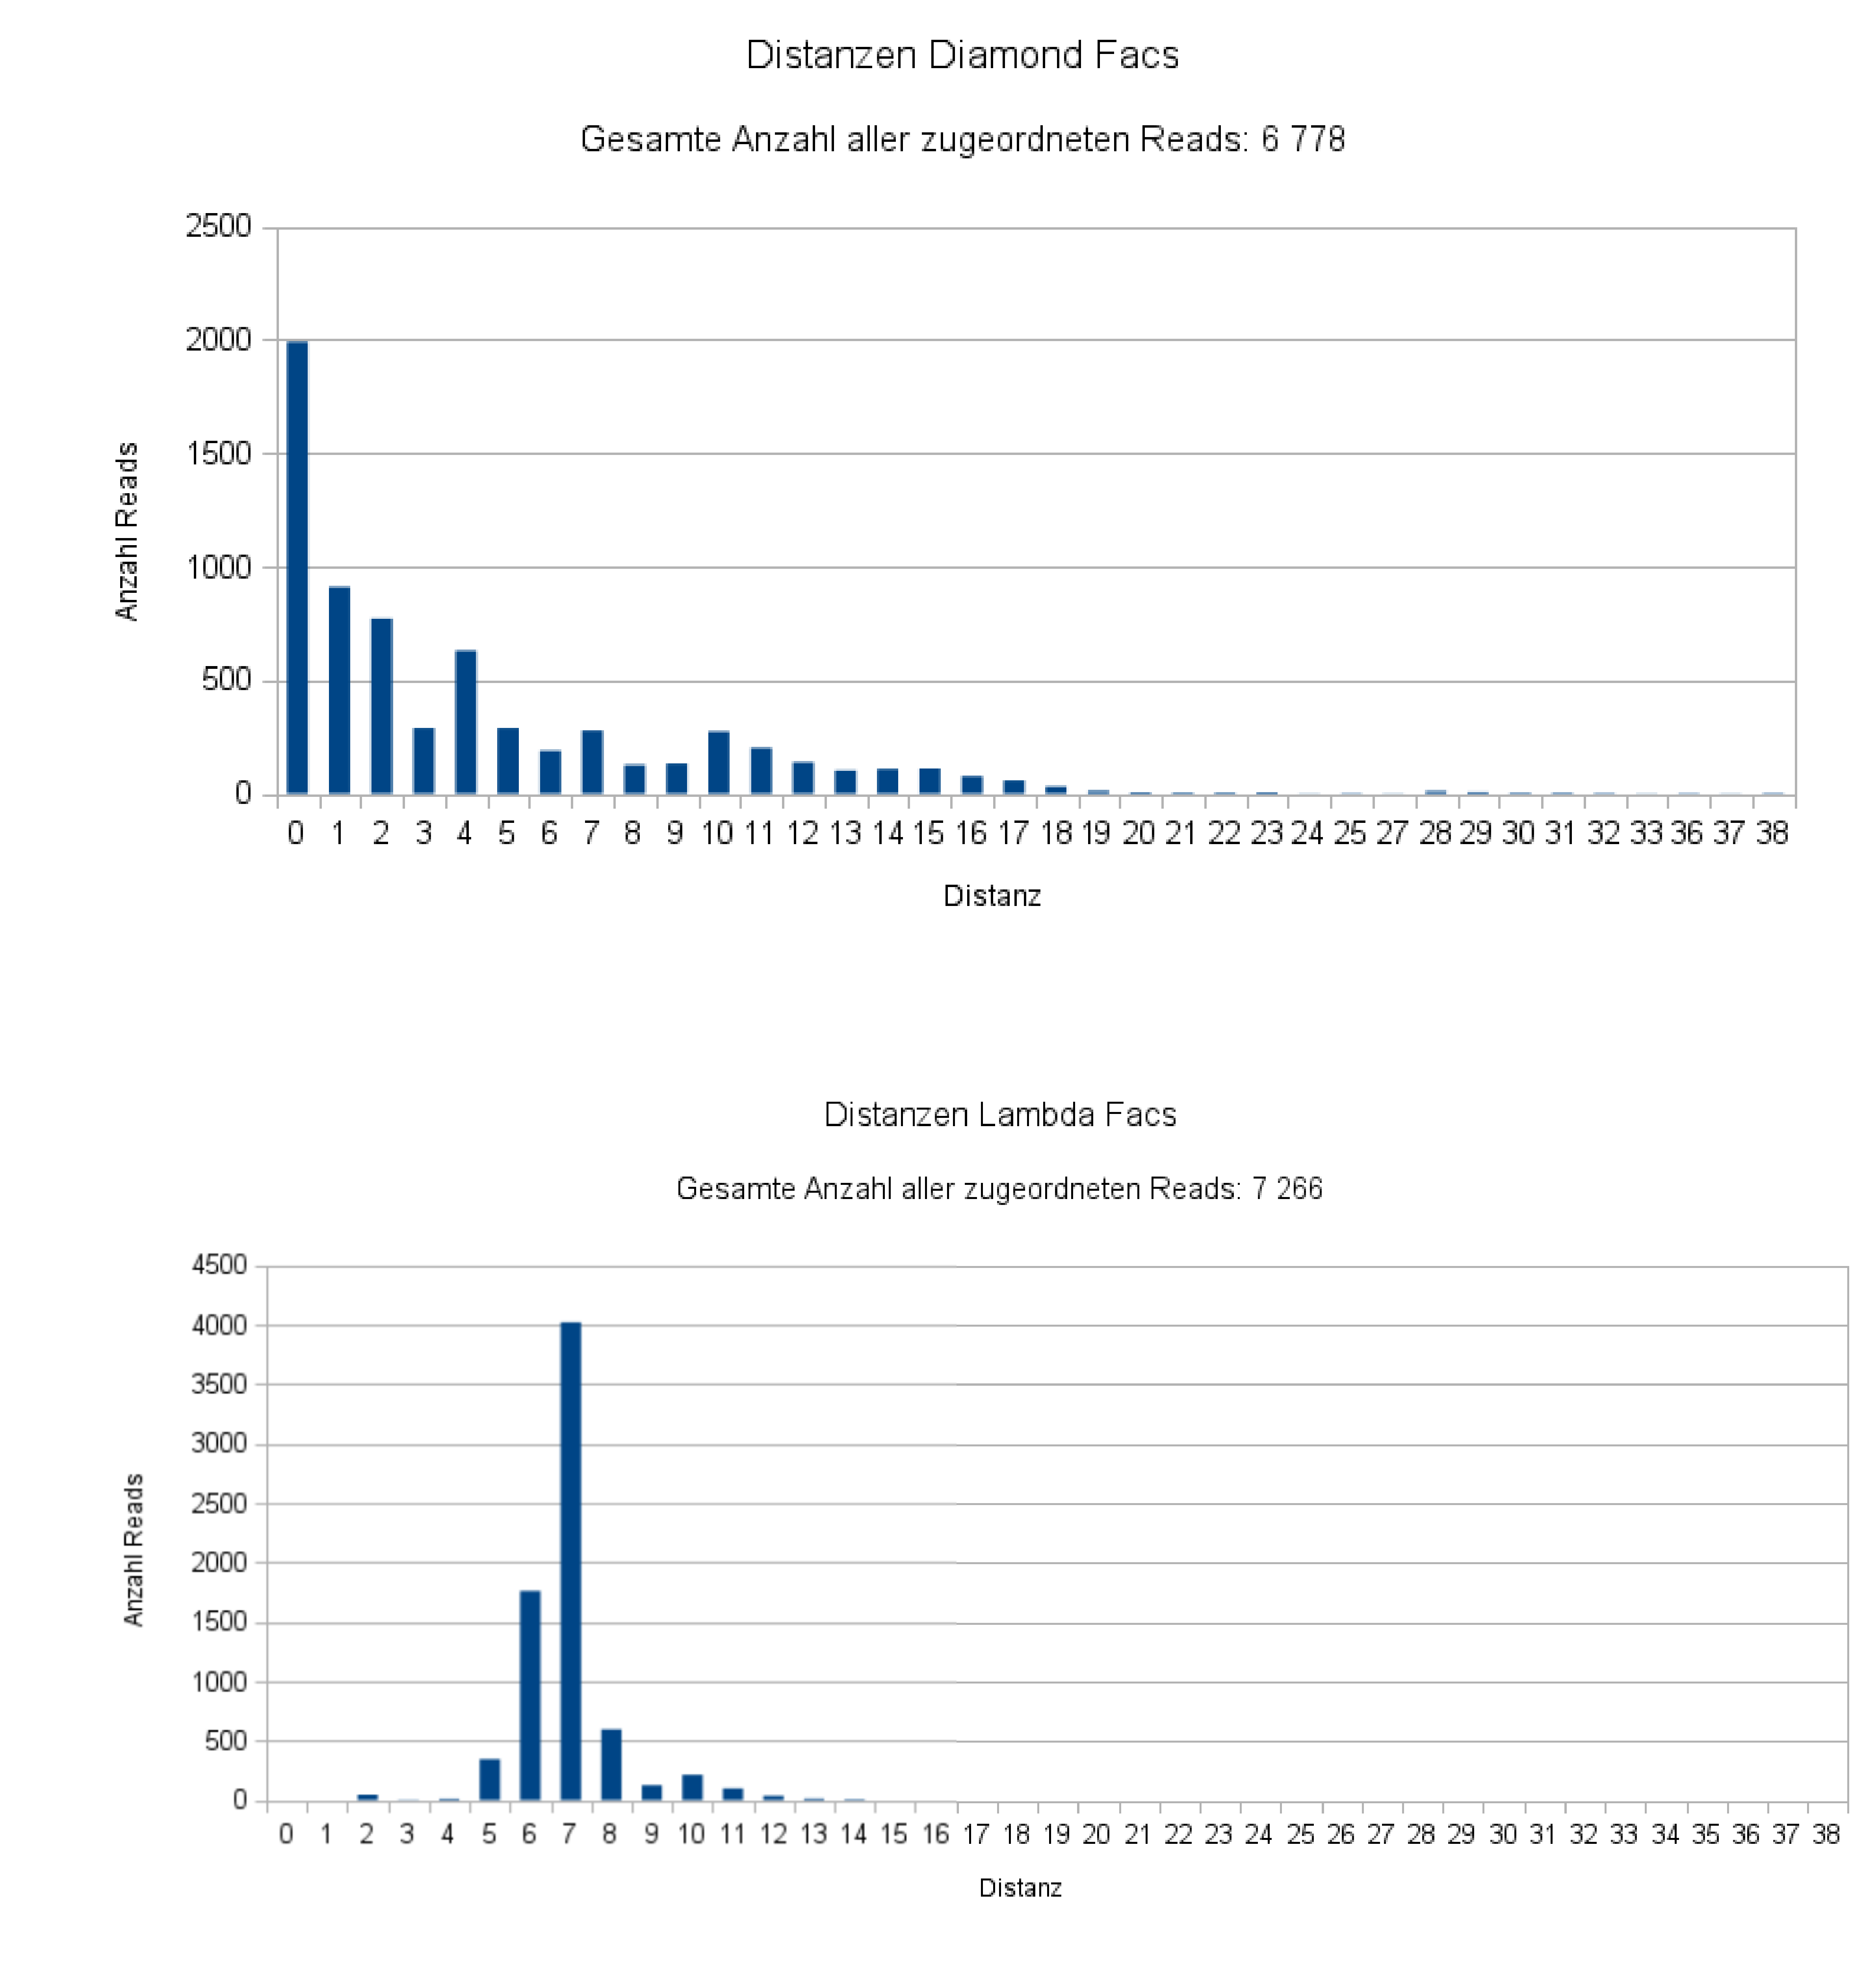
\includegraphics[width=\linewidth,height=15cm,
      keepaspectratio]{Abbildungen/Facs_Distanzen_both.png}
      \caption{Verteilung der Distanzen: Facs Datensatz}
    \end{figure}
    
     \begin{figure}[H]
      \centering
      \noindent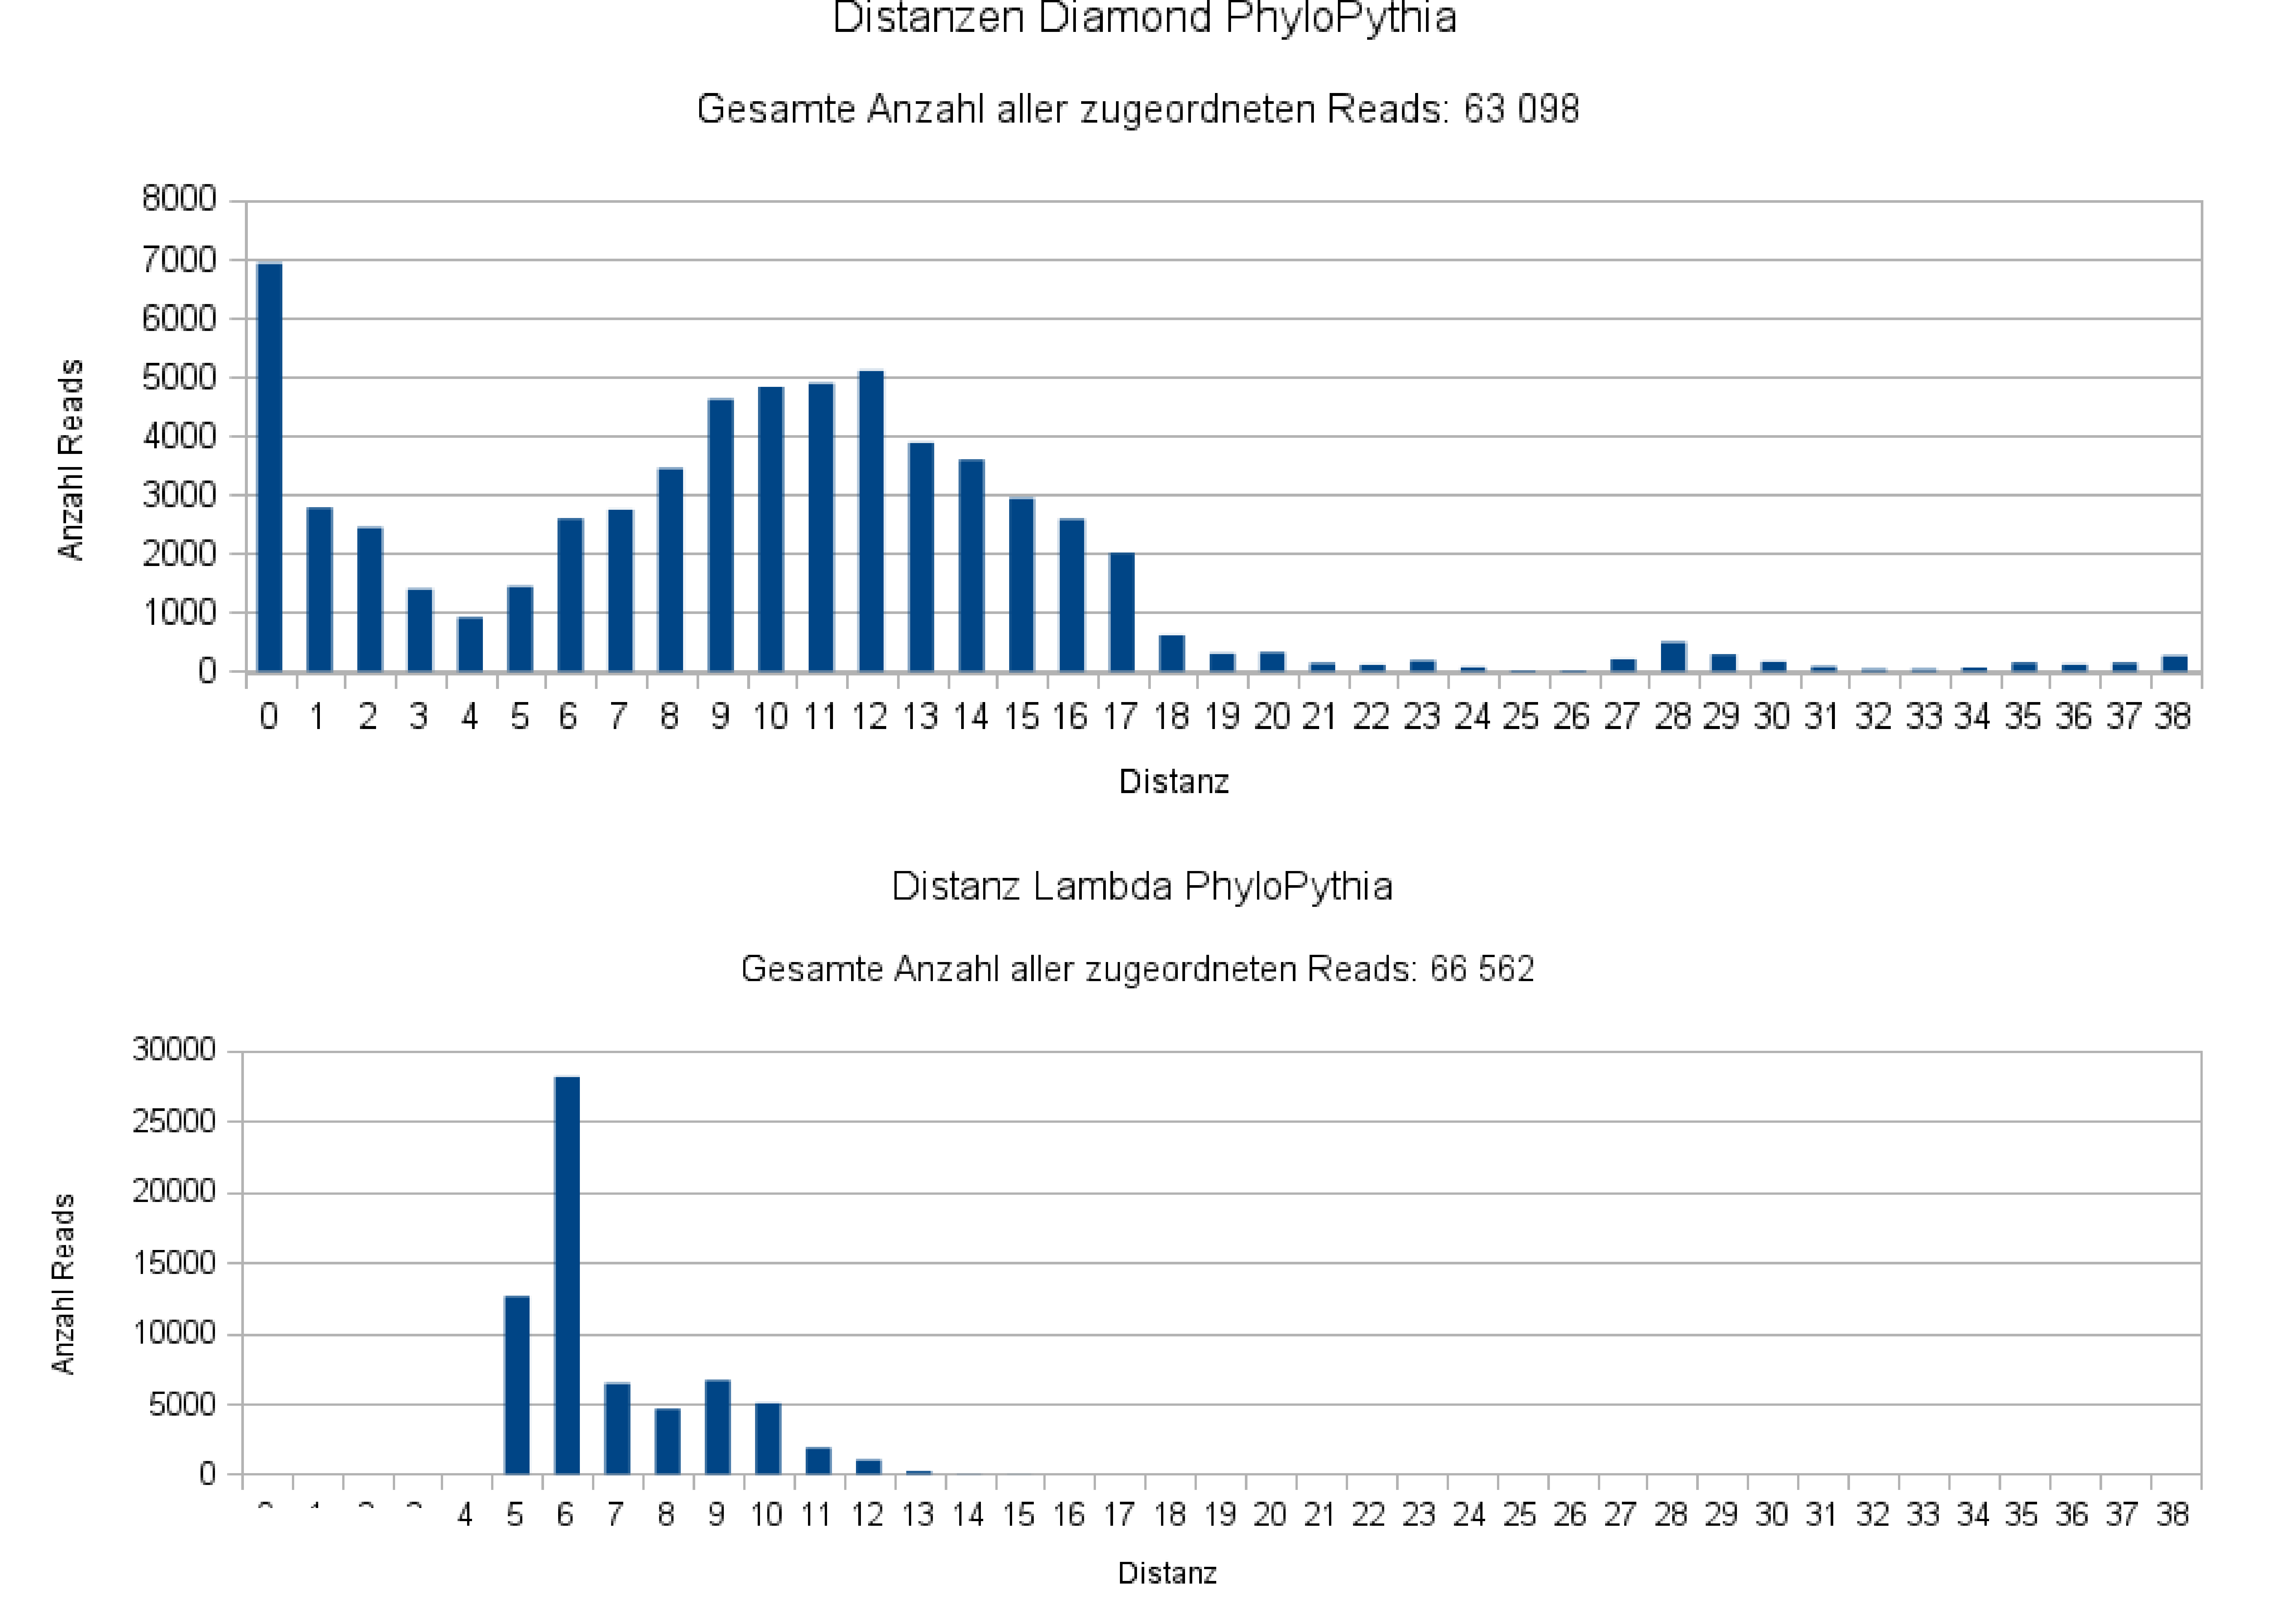
\includegraphics[width=\linewidth,height=15cm,
      keepaspectratio]{Abbildungen/PhyloPythia_Distanzen_both.png}
      \caption{Verteilung der Distanzen: PhyloPythia Datensatz}
    \end{figure}
    
    
In den \"ubrigen drei Datens\"atzen 

     \begin{figure}[H]
      \centering
      \noindent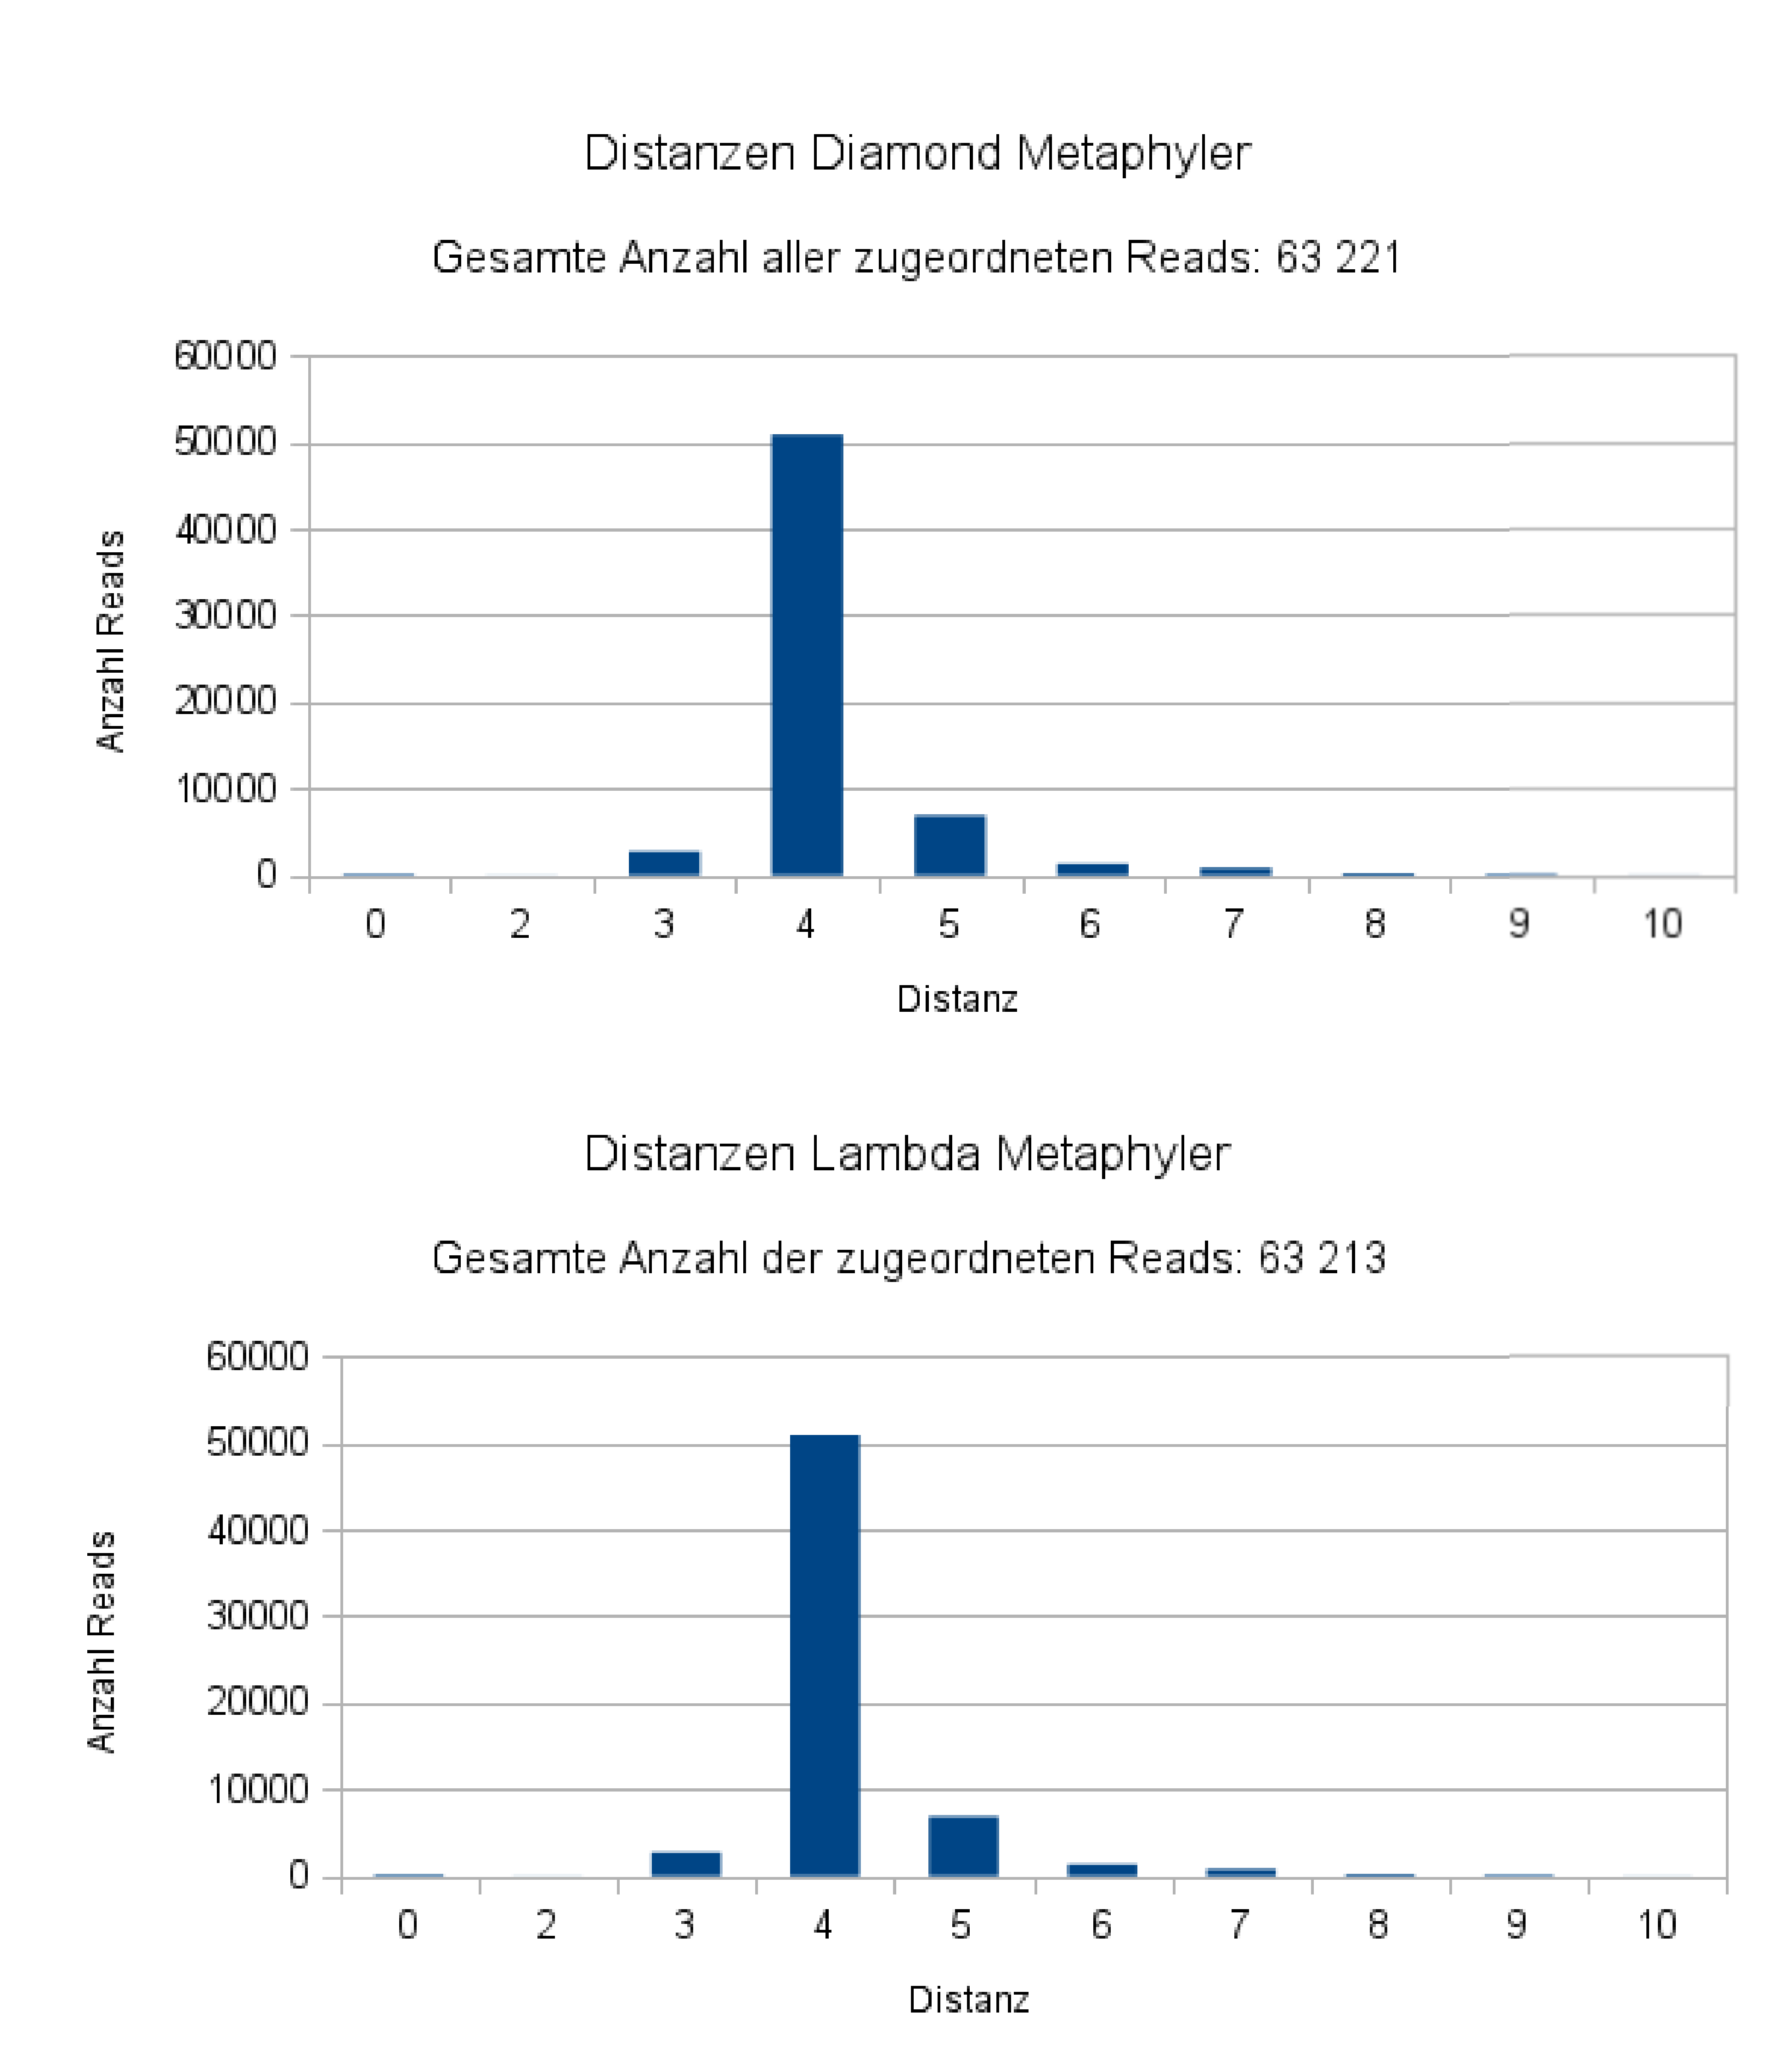
\includegraphics[width=\linewidth,height=15cm,
      keepaspectratio]{Abbildungen/Metaphyler_Distanzen_both.png}
      \caption{Verteilung der Distanzen: Metaphyler Datensatz}
    \end{figure}


     \begin{figure}[H]
      \centering
      \noindent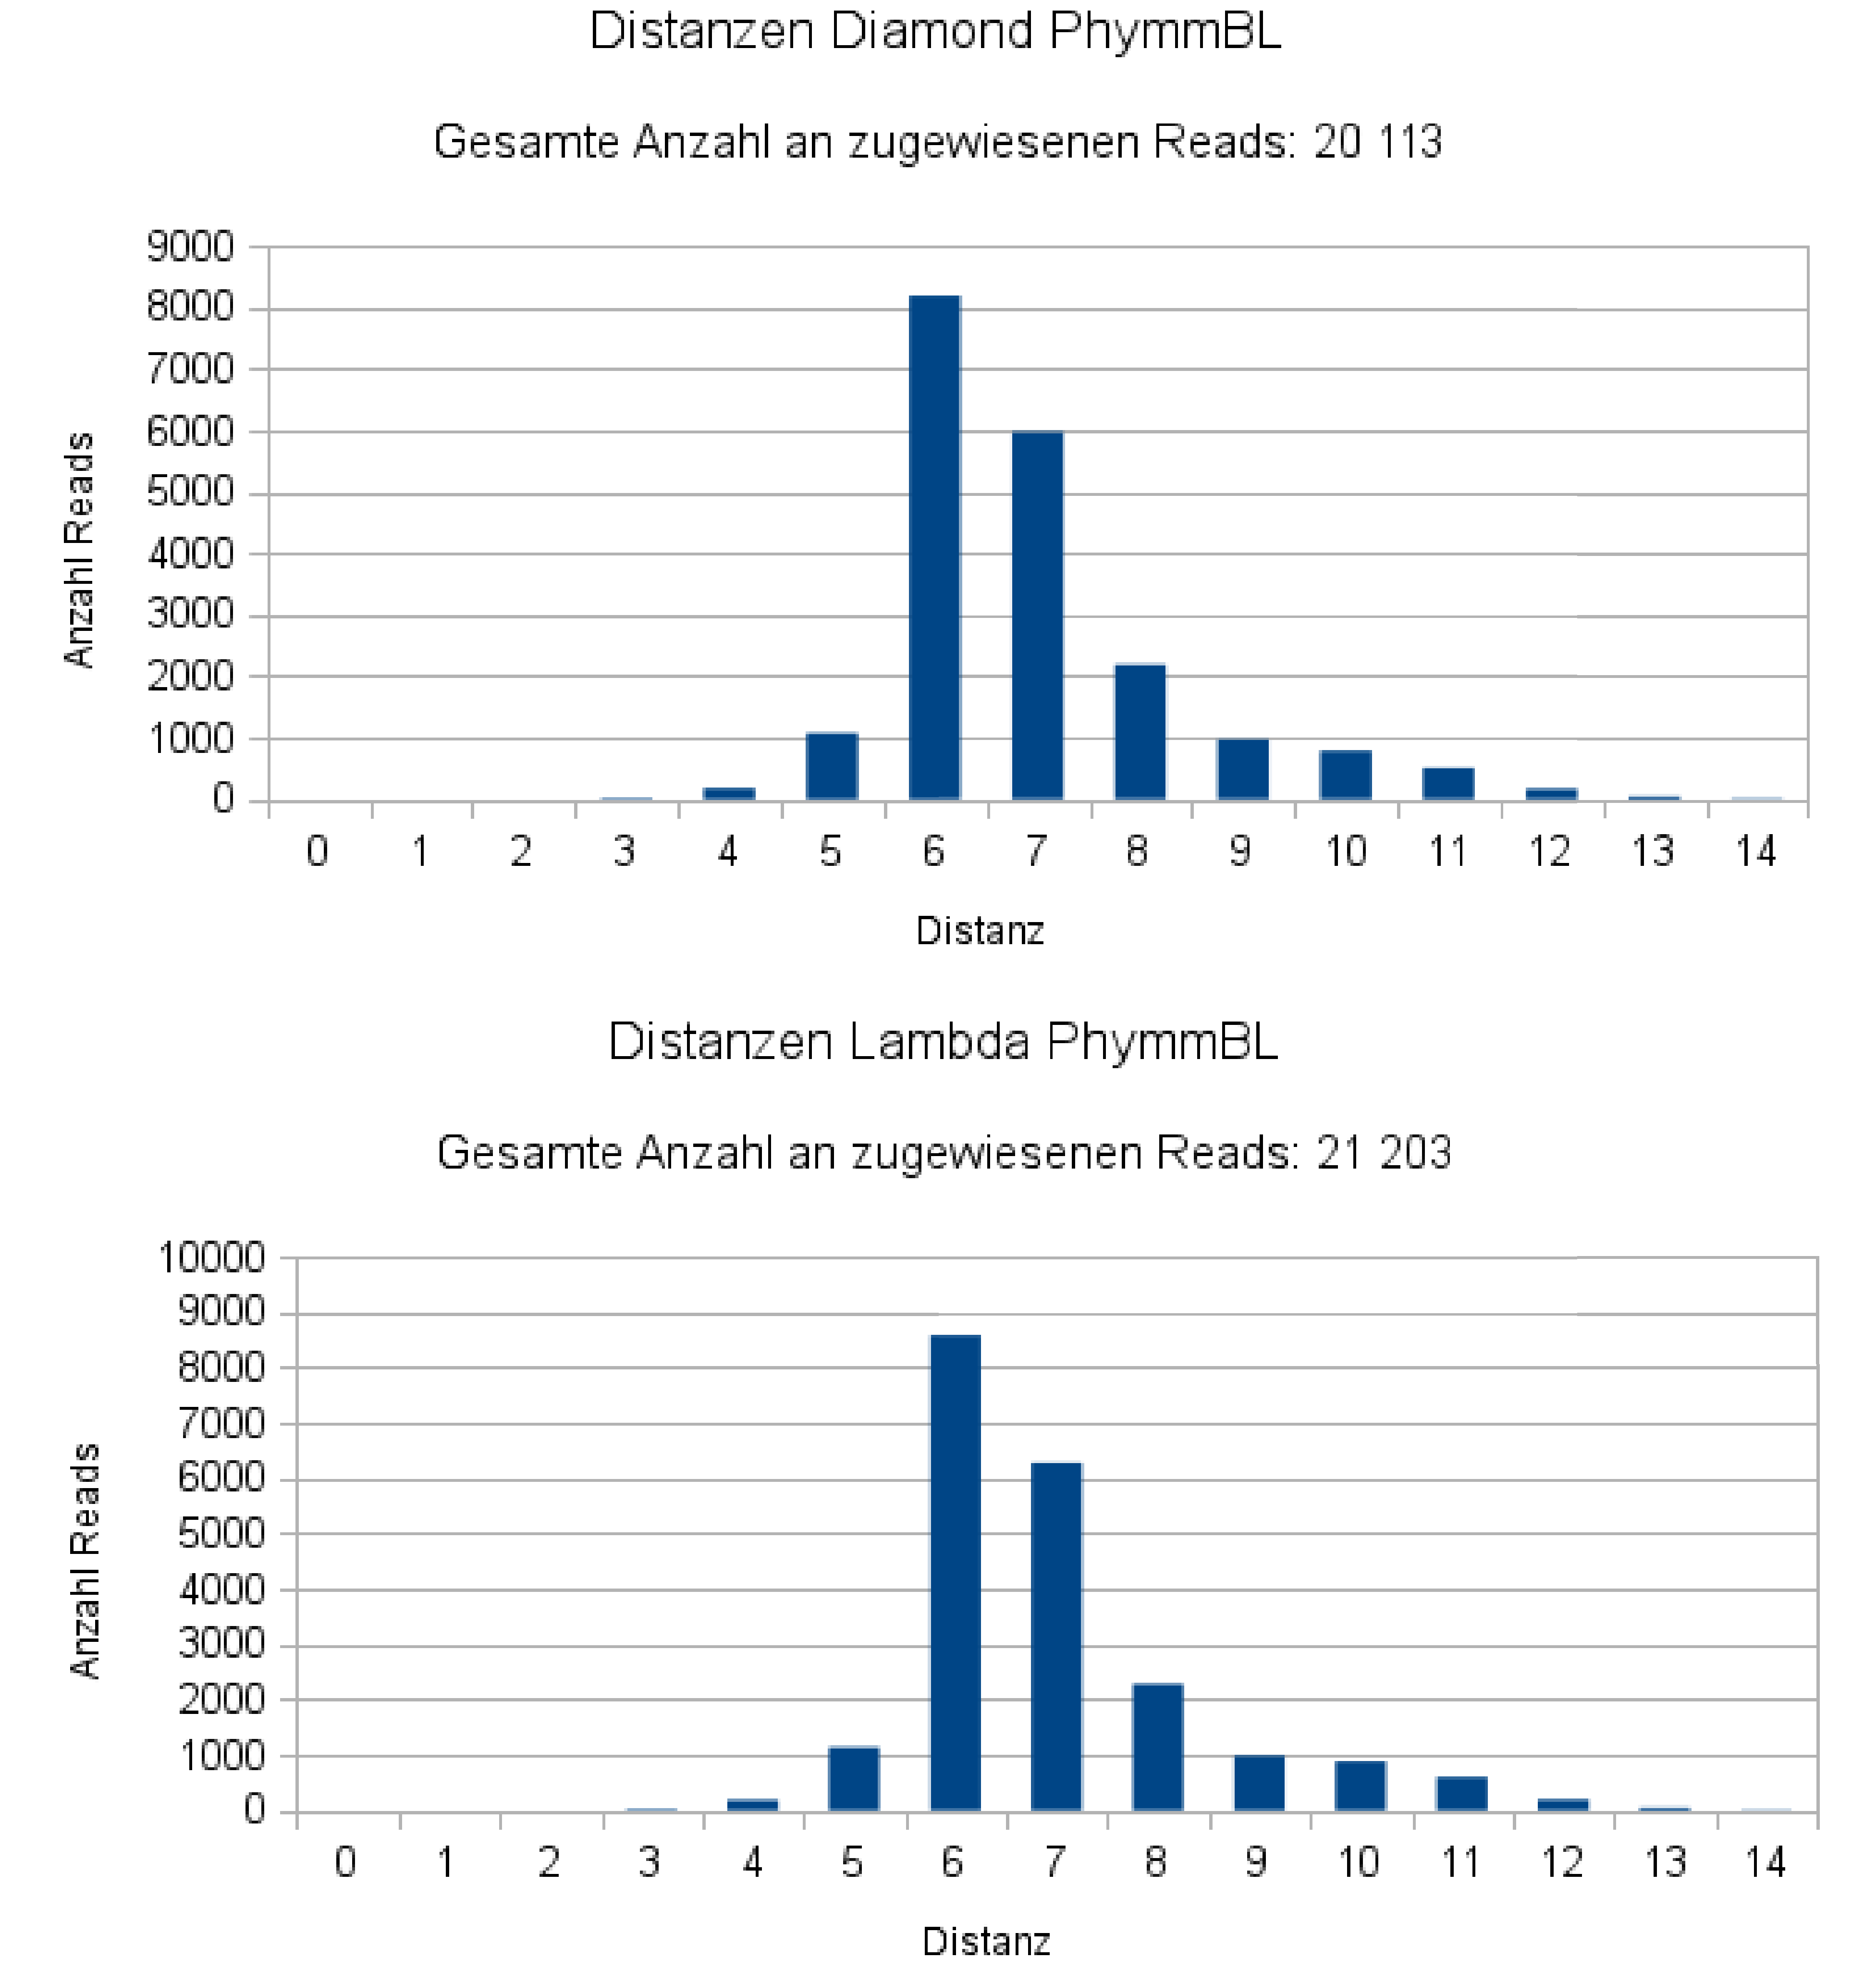
\includegraphics[width=\linewidth,height=15cm,
      keepaspectratio]{Abbildungen/PhymmBL_Distanzen_both.png}
      \caption{Verteilung der Distanzen: PhymmBL Datensatz}
    \end{figure}
    
     \begin{figure}[H]
      \centering
      \noindent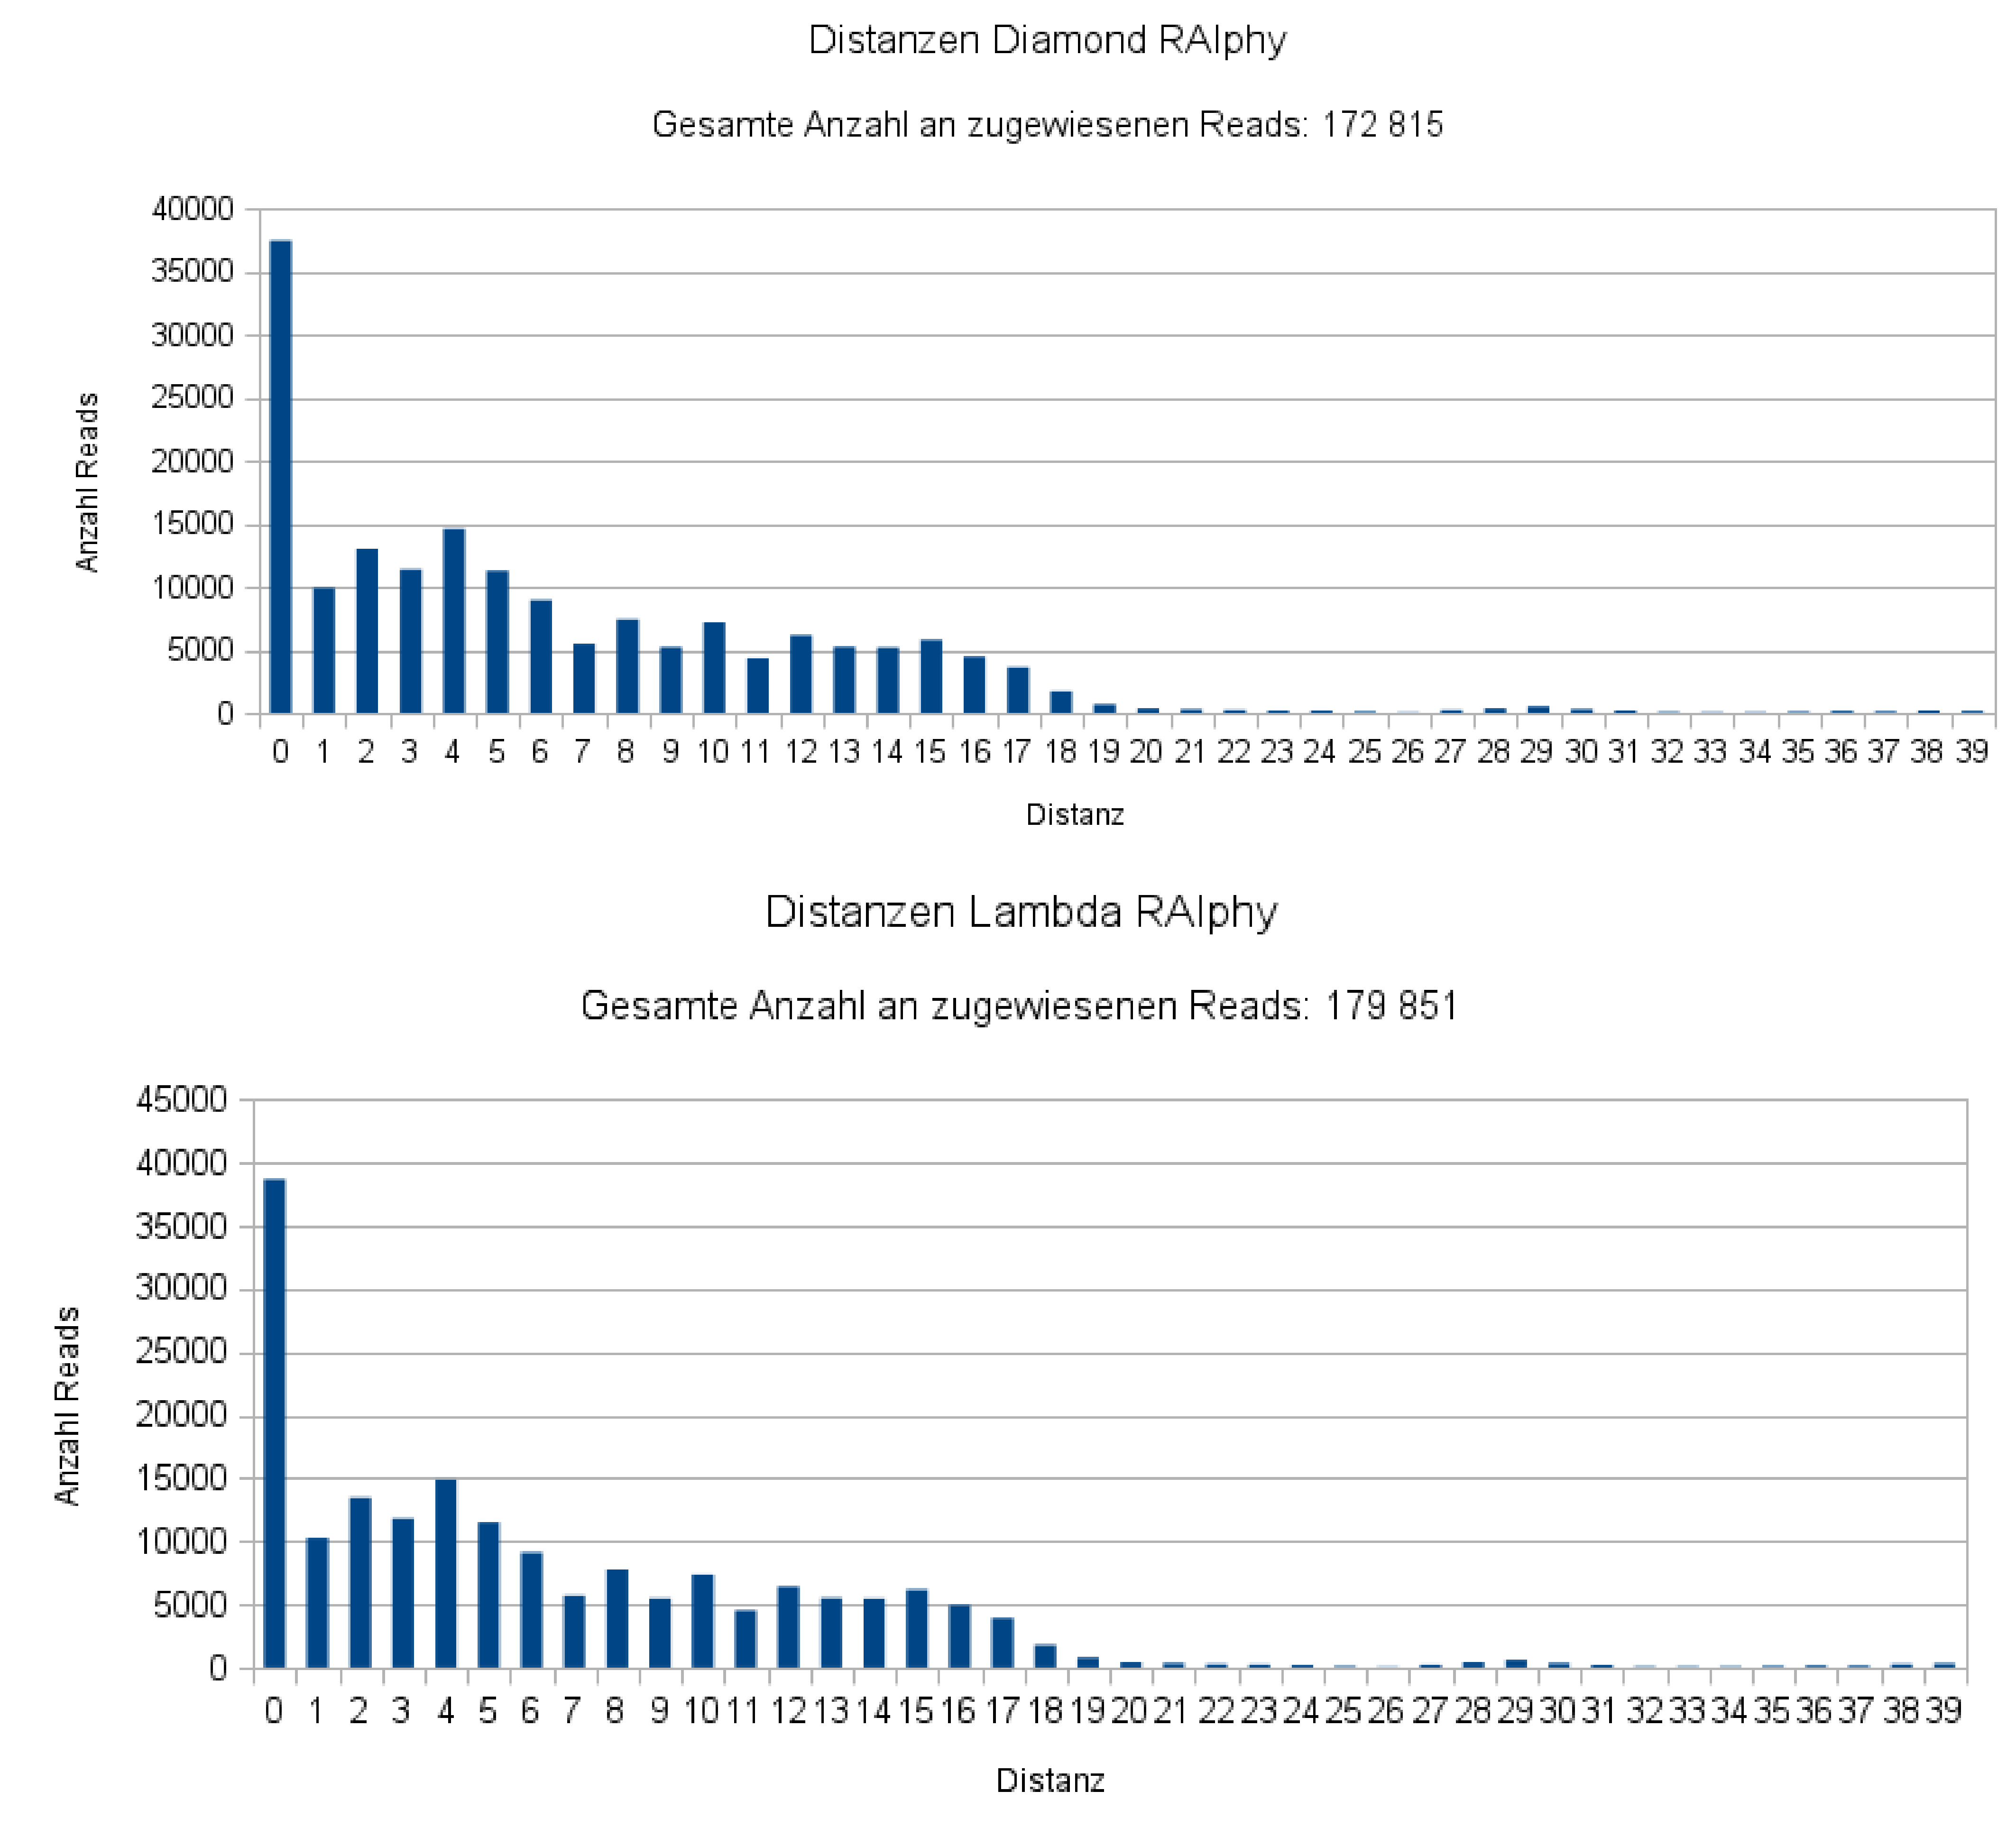
\includegraphics[width=\linewidth,height=15cm,
      keepaspectratio]{Abbildungen/RAIphy_Distanzen_both.png}
      \caption{Verteilung der Distanzen: RAIphy Datensatz}
    \end{figure}
    
    \newpage
  \section{Diskussion}
    \newpage
    \newpage
    \begin{thebibliography}{11}
    
      \bibitem{bairoch2004}
	  Bairoch, A., Boeckmann, B., Ferro, S., Gasteiger, E. 2004, Swiss-Prot: 		  juggling between evolution and stability. Brief Bioinform. 539–55
	  
	  \bibitem{bazinet2012}
	  A. L. Bazinet and M. P. Cummings. \textit{A comparative evaluation of 		  sequence classification programs}. BMC Bioinformatics, 13: p92, 2012.
	  
	  \bibitem{bradysalzberg2009}
	  Brady A, Salzberg SL: Phymm and PhymmBL: metagenomic phylogenetic 			  classification with interpolated Markov models. Nat Methods 2009, 			  6(9):673-U68. 10.1038/nmeth.1358
	  
	  \bibitem{buchfink2014}
      Buchfink B., Xie C., Huson D.H.
	  Fast and sensitive protein alignment using DIAMOND. Nat. Methods 				  2014;12:59-60.
	  
	  \bibitem{GerlachStoye2011}
	  Gerlach W, Stoye J: Taxonomic classification of metagenomic shotgun 			  sequences with CARMA3. Nucleic Acids Res 2011, 39(14):e91. 					  10.1093/nar/gkr225
  
	  \bibitem{handelsman1998} 
      Jo Handelsman, Michelle R. Rondon, Sean F. Brady, Jon Clardy and Robert   	  M.Goodman. \textit{Molecular biological access to the chemistry of 			  unknown soil microbes: a new frontier for natural products}. Chemistry \& 	  Biology, 5(10): 245-249, 1998.
      
      \bibitem{hauswedell2014}
      Lambda: the local aligner for massive biological data; Hannes Hauswedell, 	  Jochen Singer, Knut Reinert; Bioinformatics 2014 30 (17): i349-i355; doi: 	  10.1093/bioinformatics/btu439
      
      \bibitem{Liu2010}
	  Liu B, Gibbons T, Ghodsi M, Pop M: MetaPhyler: Taxonomic profiling for 		  metagenomic sequences. In IEEE International Conference on Bioinformatics 	  and Biomedicine (BIBM). , Hong Kong; 2010:95–100.
	  
	  \bibitem{nalbantoglu2011}
	  Nalbantoglu OU, Way SF, Hinrichs SH, Sayood K: RAIphy: phylogenetic 			  classification of metagenomics samples using iterative refinement of 			  relative abundance index profiles. BMC Bioinf 2011, 12: 41. 					  10.1186/1471-2105-12-41
	  
	  \bibitem{patil2011}
	  Patil KR, Haider P, Pope PB, Turnbaugh PJ, Morrison M, Scheffer T, 			  McHardy AC: Taxonomic metagenome sequence assignment with structured 			  output models. Nat Methods 2011, 8(3):191–192. 10.1038/nmeth0311-191
		 
	  
	  \bibitem{stranneheim2010}
	  Stranneheim H, Kaller M, Allander T, Andersson B, Arvestad L, Lundeberg 		  J: Classification of DNA sequences using Bloom filters. Bioinformatics 		  2010, 26(13):1595–1600. 10.1093/bioinformatics/btq230
	  
	  

    \end{thebibliography}


\end{document}




